
\chapter{面向模型推理的云边协同调度方法}

本章系统地阐述了面向模型推理的云边协同调度。首先,详细介绍了云边协同下的模型推理,包括云边协同系统的拓扑结构、模型推理的云边协同场景,以及分层拓扑下的委托推理流程。基于抽象的树状拓扑结构,本文提出了一种面向模型推理的云边协同调度模型,并设计了相应的调度算法,以优化资源利用和任务执行效率。

\section{云边协同下的模型推理}

\subsection{云边协同系统拓扑结构}

云边协同的核心目标在于通过协调跨层级资源,以尽可能高效地满足物联网(IoT)设备的数据处理需求。为了实现IoT设备数据的高效采集,并提供灵活且高效的接入能力,现有框架通常借助抽象层来屏蔽底层硬件差异,进而为异构终端设备提供标准化的接入接口。例如,KubeEdge\cite{xiong2018extend}通过设备孪生(Device Twin)技术建立物理设备的数字镜像,支持基于标准MQTT协议接入工业传感器、智能摄像头等终端设备,其双向同步机制可保证设备状态与云端视图的一致性;Tango\cite{bagchi2017tango}则提出分层设备管理模型,通过边缘代理层(Edge Proxy)对Modbus、CAN总线等工业协议进行转换,为低功耗嵌入式设备提供资源虚拟化接口。若缺乏此类模块,开发人员则需自行实现设备协议解析、数据格式转换等底层适配逻辑,实现设备管理器,才能读取相关数据。

\begin{figure}[ht]
  \centering
  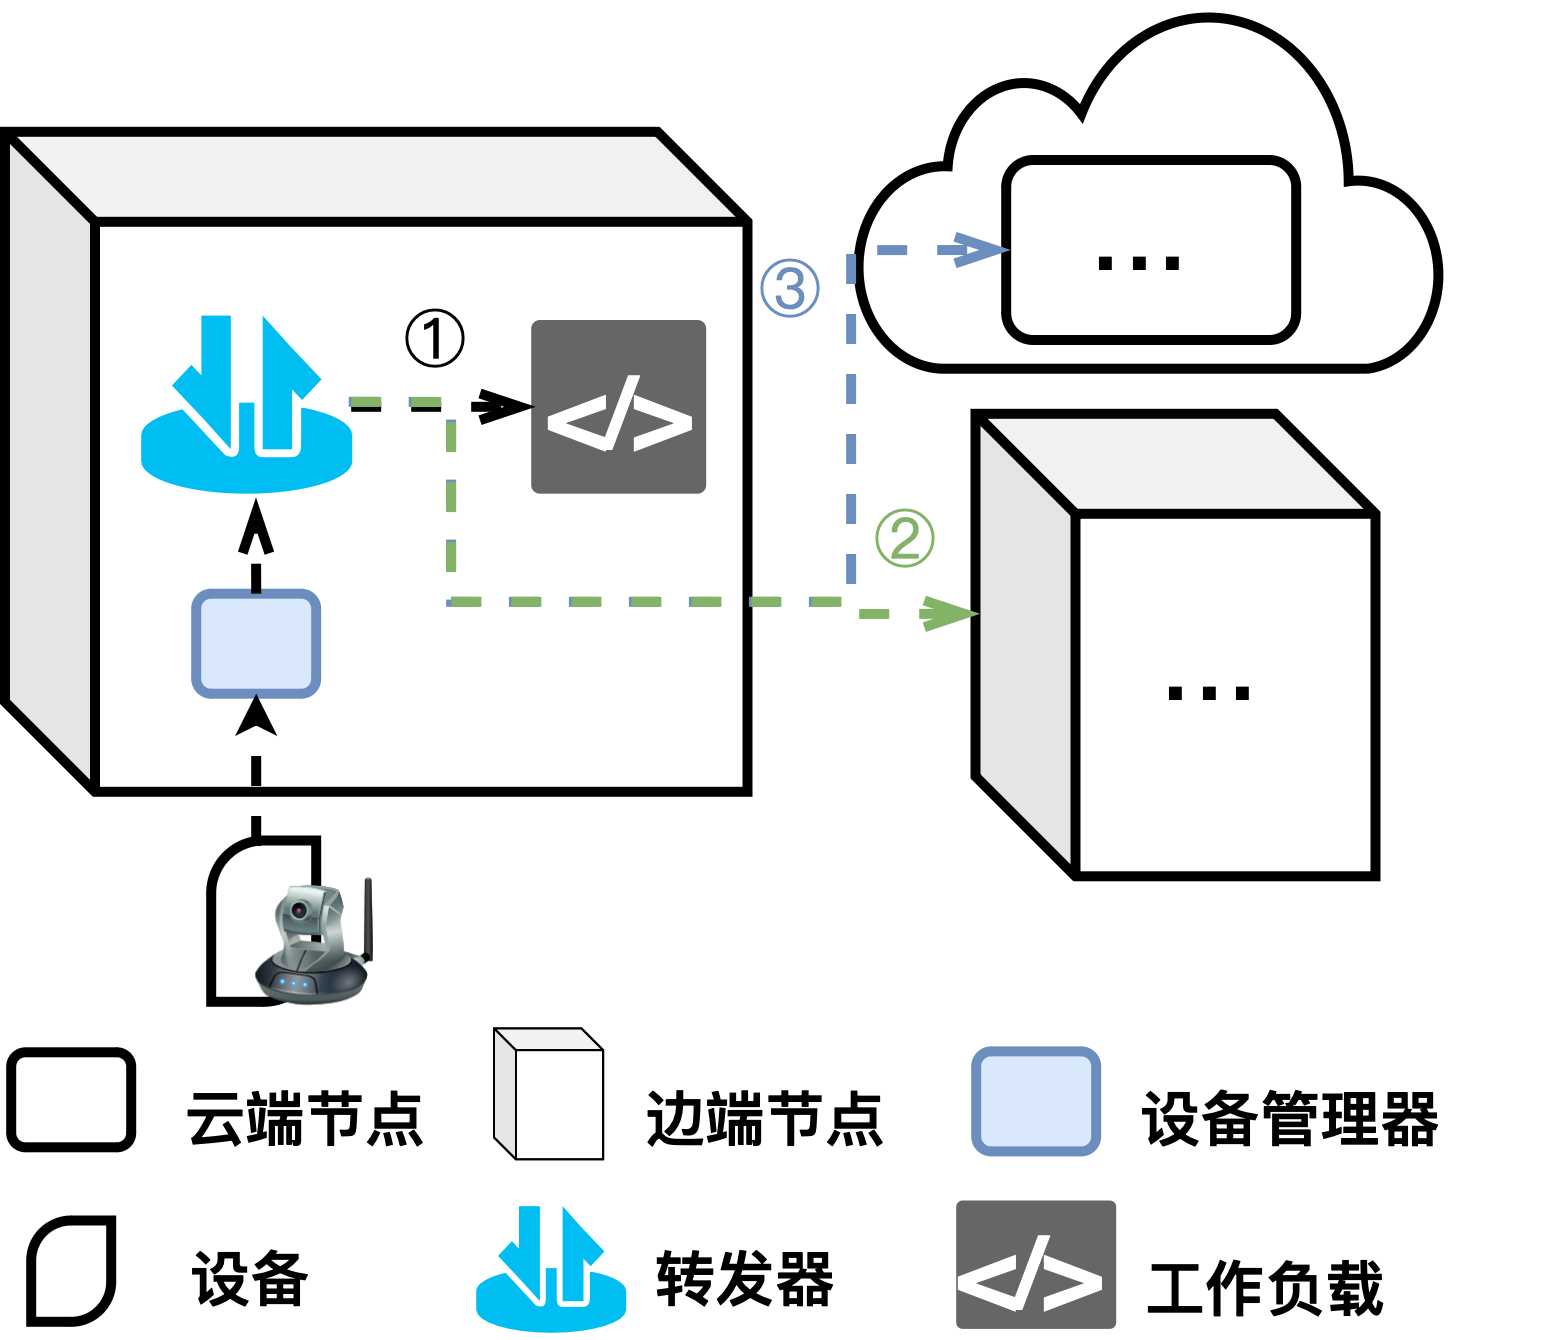
\includegraphics[width=0.45\linewidth]{pics/3-1流处理.png}
  \caption{流式数据调度与多级协作}
  \label{fig:3-1flow}
\end{figure}

IoT设备产生的时序数据具有连续性强、时间敏感性高的特点,因此适合采用流处理范式进行实时处理\cite{de2018distributed,wang2020edge}。如图\ref{fig:3-1flow}所示,云边平台可根据负载状态,对于流式时序数据实现调度决策,既可以在本地边缘节点直接执行,也可以转发至其他边缘节点以实现水平方向的协作,或者依托云端全局视图实现云边节点间的跨层级垂直协作。目前,部分边端流处理框架已初步支持轻量级数据过滤与转发功能。例如,Kuiper\cite{ekuiper}通过SQL-like语法定义数据过滤规则,能够对原始数据进行实时过滤与简单转换,并将结果转发至其他节点,但尚未集成智能化的动态调度决策机制。这些引擎主要面向基于阈值的轻量级计算任务,尽管部分框架尝试适配AI推理功能,但尚未充分解决云边异构化环境下AI推理任务的部署问题,缺乏对深度学习框架版本冲突的兼容性保障以及跨架构硬件适配机制。

\begin{figure}[ht]
  \centering
  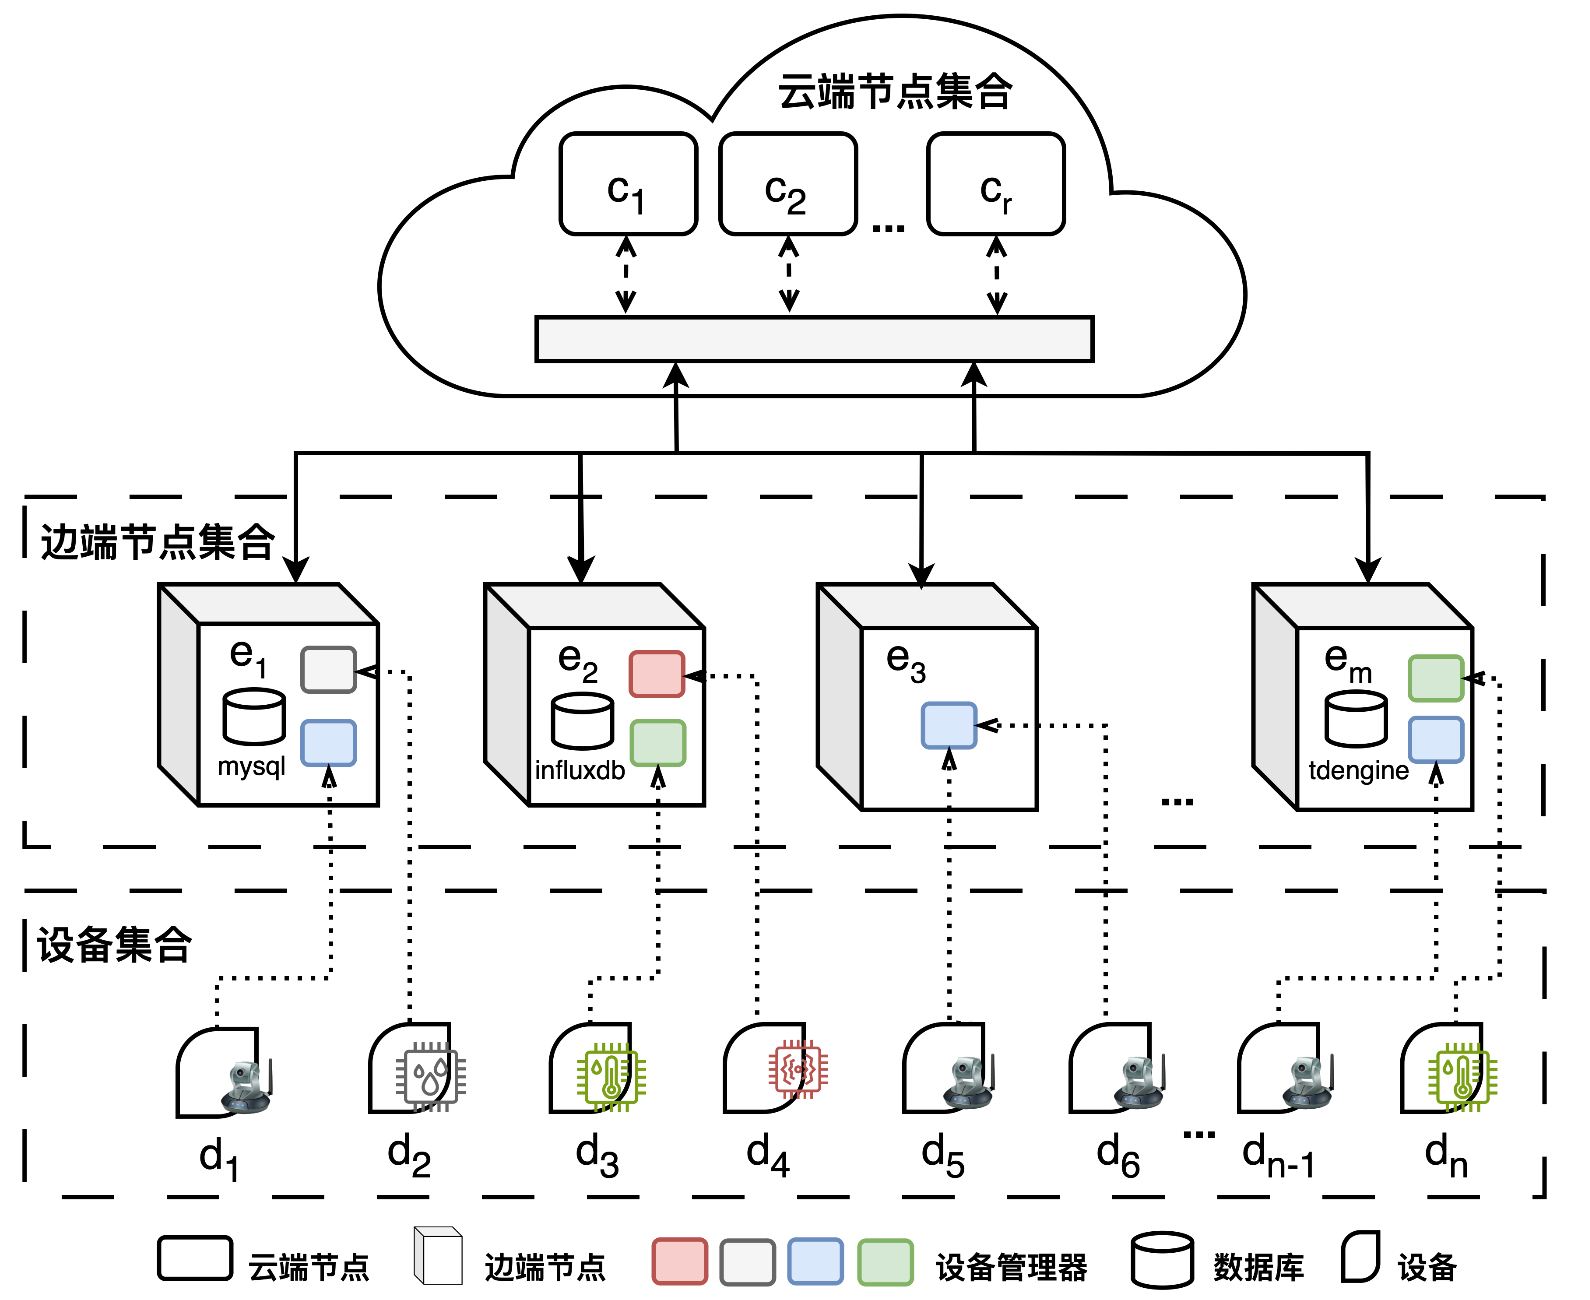
\includegraphics[width=0.9\linewidth]{pics/3-2模型架构.png}
  \caption{云边协同物理拓扑}
  \label{fig:3-2model}
\end{figure}

如图\ref{fig:3-2model}所示,云边协同的分层设计为上述功能提供了基础支撑。该架构在物理上由设备层、边缘节点层和云端节点层组成。其中,设备层由各类IoT终端设备构成,负责感知环境并生成原始数据流;边缘节点层位于设备层与云端之间,作为中间层承担了任务卸载、数据预处理及局部决策等功能,从而有效减轻云端的压力并降低系统延迟;云端节点层则提供了全局视角和强大的计算能力,用于执行复杂任务、存储大规模数据以及制定全局优化策略。

在此基础上,本文进一步探讨计算节点的层次结构。云端节点通常具备强大的计算能力和存储资源,适合处理复杂、计算密集型任务。相比之下,位于终端设备与云端之间的边缘层由多级边缘节点组成,这些节点逻辑上同样呈现分层结构,能够根据其位置和能力承担不同程度的计算任务。例如,靠近终端设备的边缘节点可能专注于实时性要求较高的轻量级任务,而更接近云端的边缘节点则可以处理相对复杂的任务或作为数据汇聚点。这种分层结构确保了系统的灵活性和高效性,使得任务能够在不同层级间动态调度,从而在资源利用率和响应速度之间达到平衡。

\begin{figure}[ht]
  \centering
  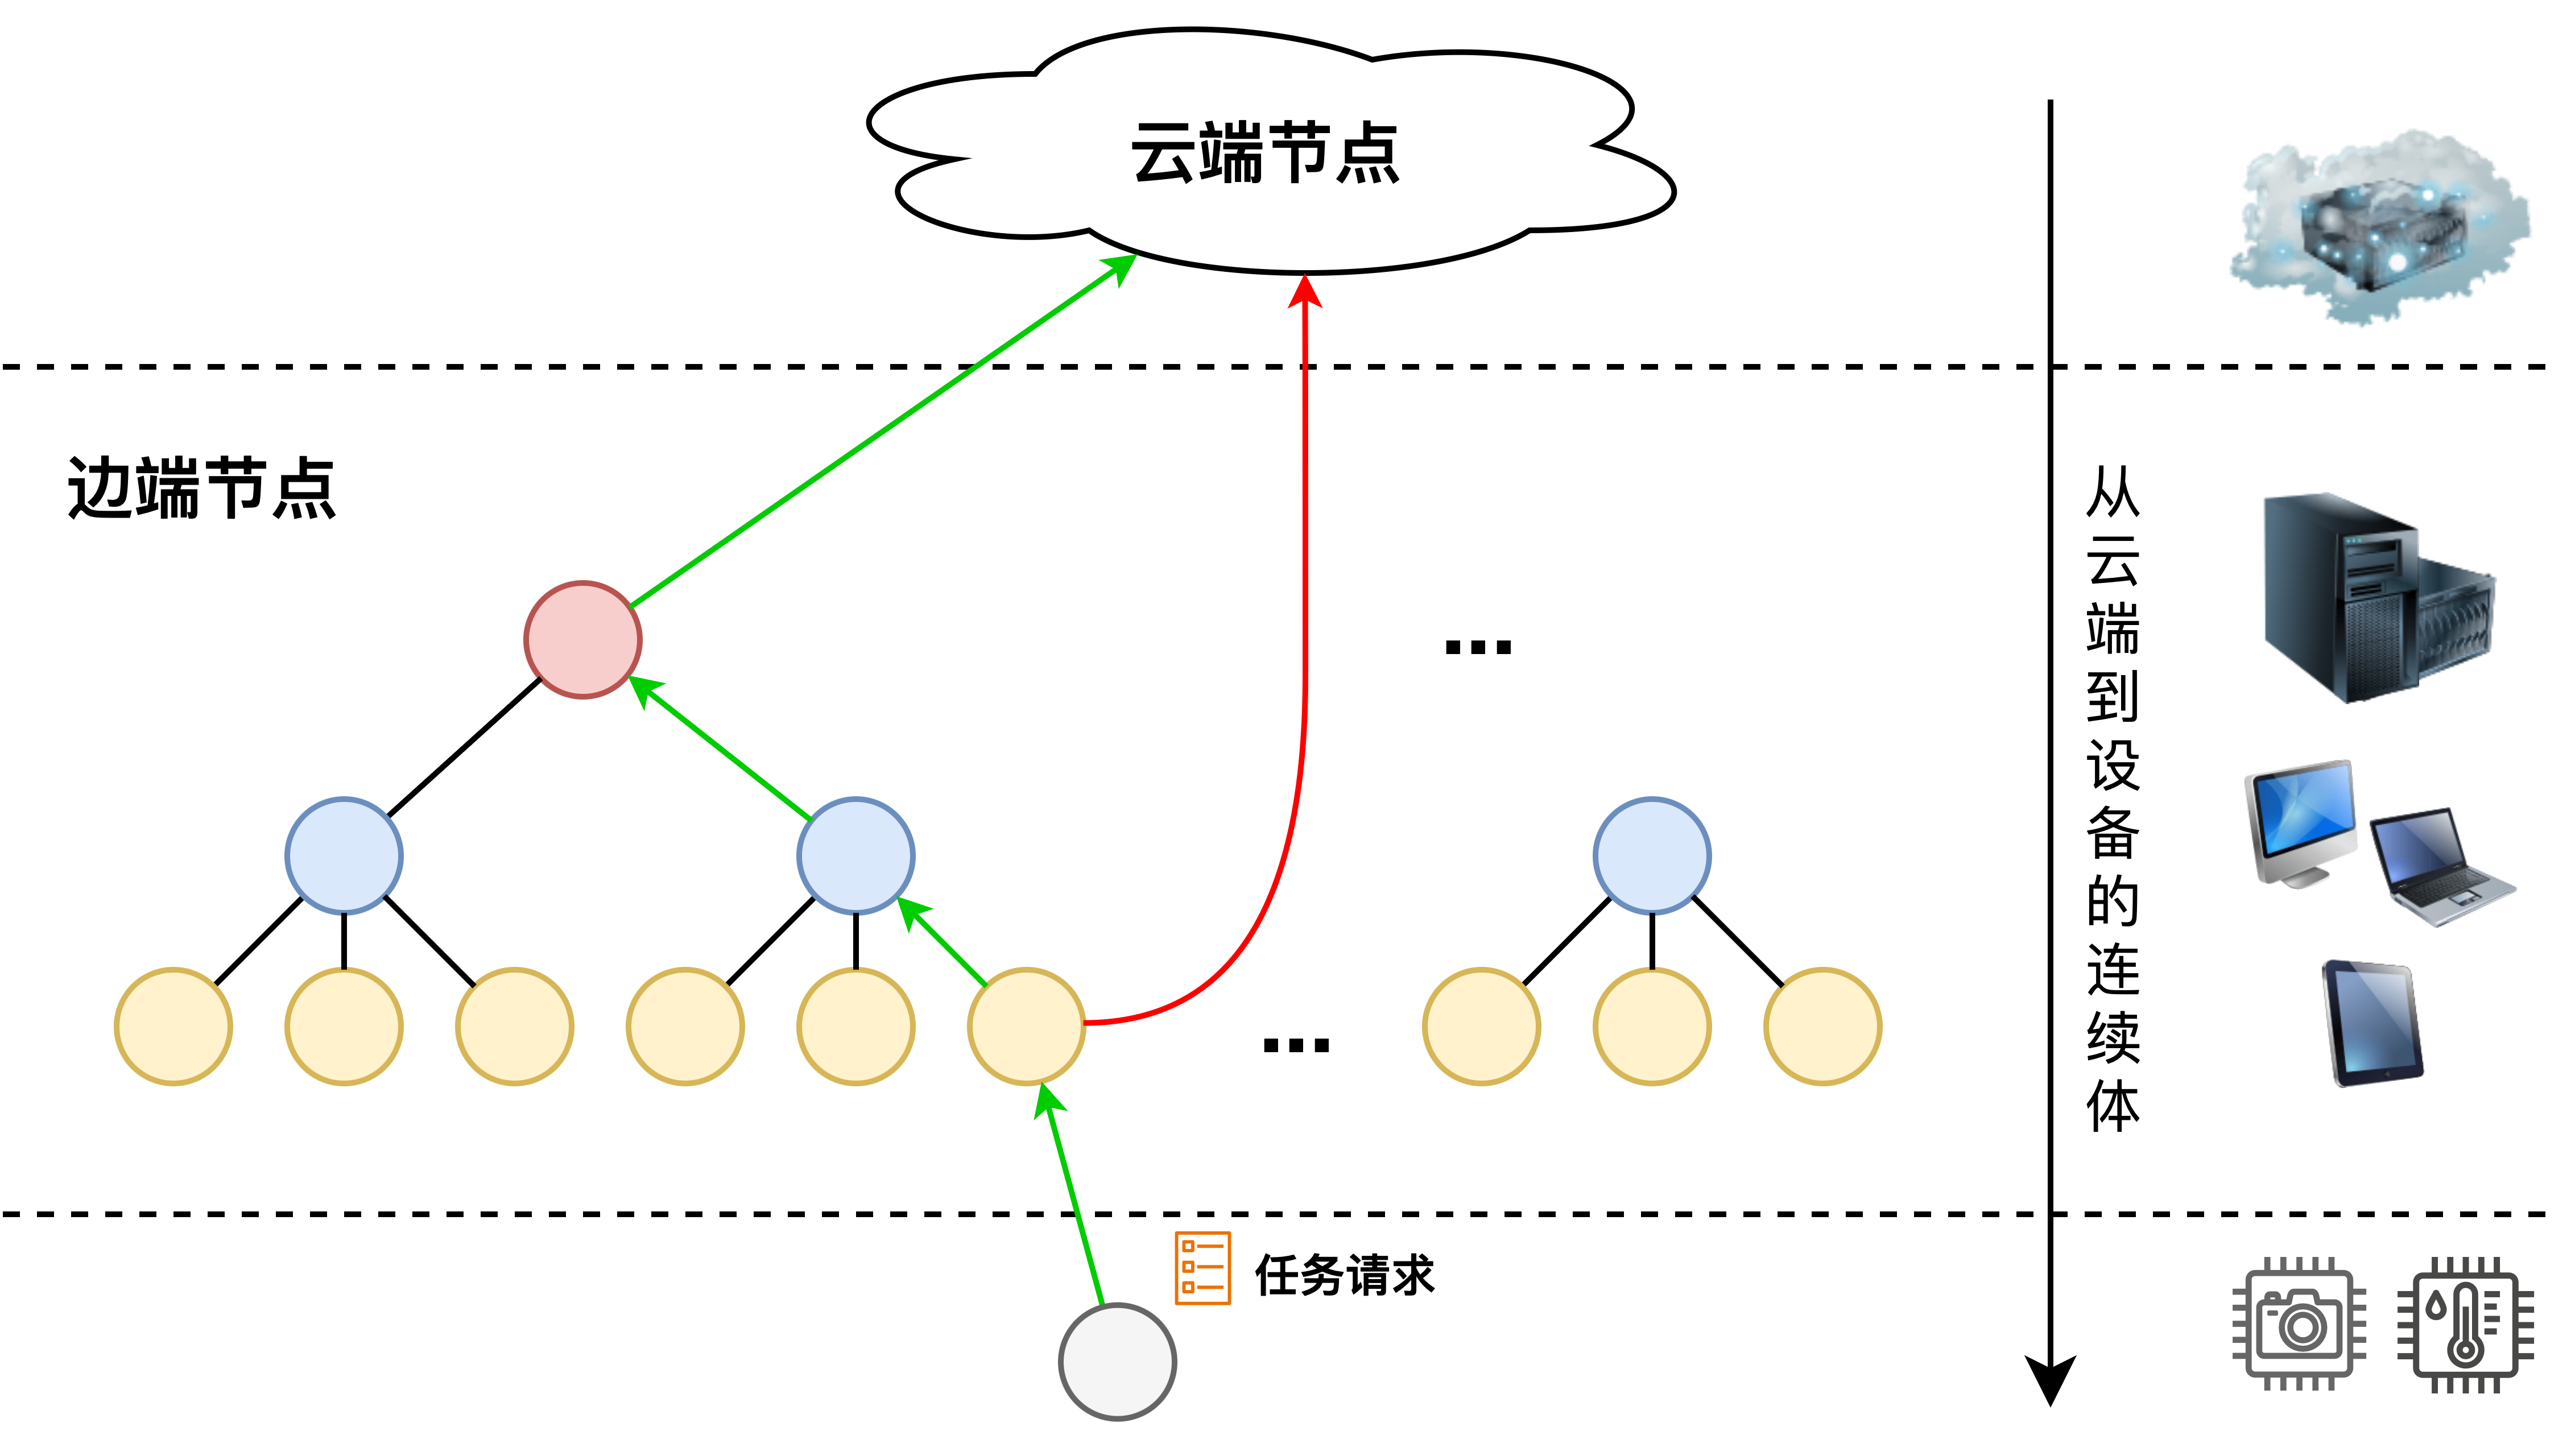
\includegraphics[width=0.8\linewidth]{pics/3-5schedule.png}
  \caption{云边协同下的树状拓扑}
  \label{fig:3-5schedule}
\end{figure}

图\ref{fig:3-5schedule}展示了这种层次化的结构,其中所有边缘节点与云端之间形成了一个树状拓扑关系。在这种树状拓扑中,云端作为根节点,负责全局资源管理和复杂任务分配,而各级边缘节点则作为分支节点,根据其位置和功能分工协作。这种设计简化了管理和通信路径,显著提升了系统的可扩展性和容错能力。即使部分边缘节点发生故障,系统仍可通过其他路径继续运行,确保整体性能不受重大影响。

\subsection{模型推理的云边协同场景}

在云边协同的推理场景中,AI推理实例的核心功能是处理IoT设备(如传感器、摄像头等)生成的实时流数据。这些设备以高频率和多样化形式持续生成数据流,例如环境监测中的温度、湿度数据或视频监控中的图像帧序列。如图\ref{fig:3-3device}所示,为了高效管理与处理这些数据,开发人员需将IoT设备注册到云边平台,并为每台设备开发对应的设备管理器。设备管理器不仅负责适配IoT设备的通信协议,从而确保平台能够接收并转译设备生成的数据格式,而且能够控制IoT设备按照指定的采集频率进行数据采集,进而满足不同应用场景对数据时效性和精度的需求。

\begin{figure}[ht]
  \centering
  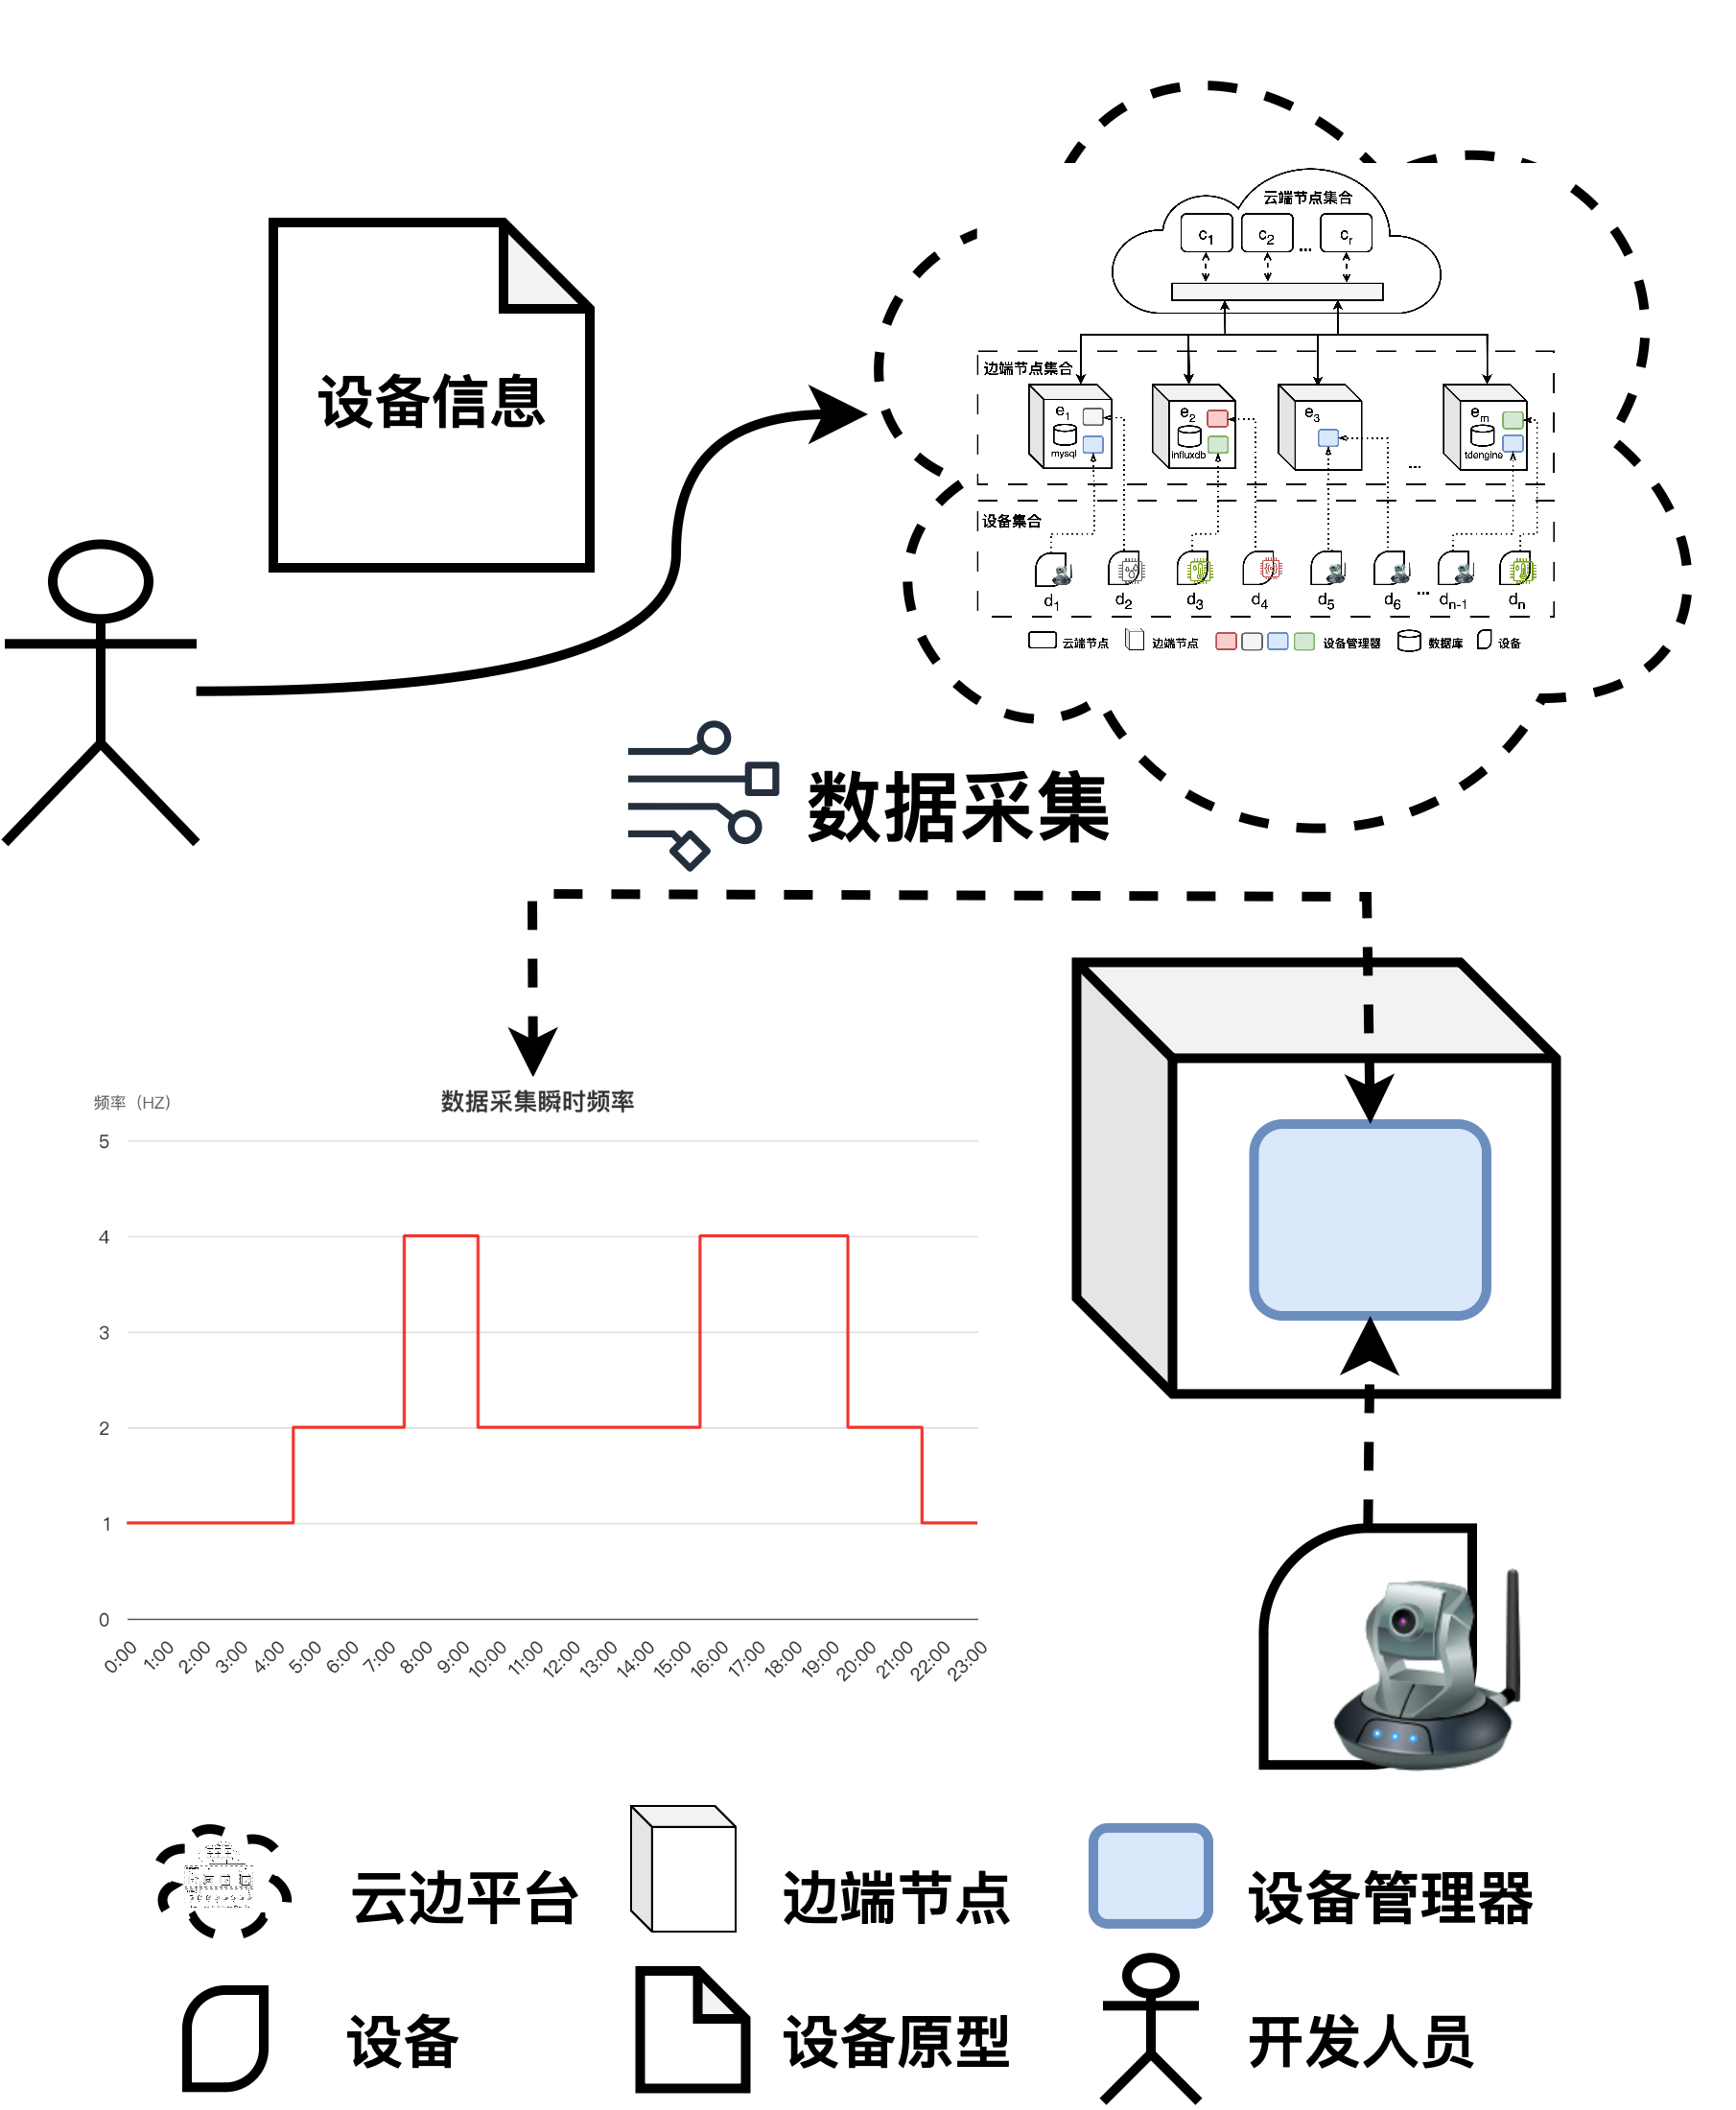
\includegraphics[width=0.6\linewidth]{pics/3-3设备模型.png}
  \caption{设备数据采集流程图}
  \label{fig:3-3device}
\end{figure}

这些原始数据通常需要经过预处理才能被AI推理实例有效利用。由于不同类型的终端设备生成的数据格式和特性存在显著差异,其预处理需求也呈现出多样化的特点。例如,视觉设备采集的图像数据可能需要进行压缩、分辨率调整或格式转换以适应存储和传输需求;而传感器设备生成的数值型数据则可能需要滤波以去除噪声干扰,或者通过归一化处理来统一量纲和范围。此外,某些场景下还可能涉及特征提取或数据聚合等更复杂的预处理操作。

\begin{figure}[ht]
  \centering
  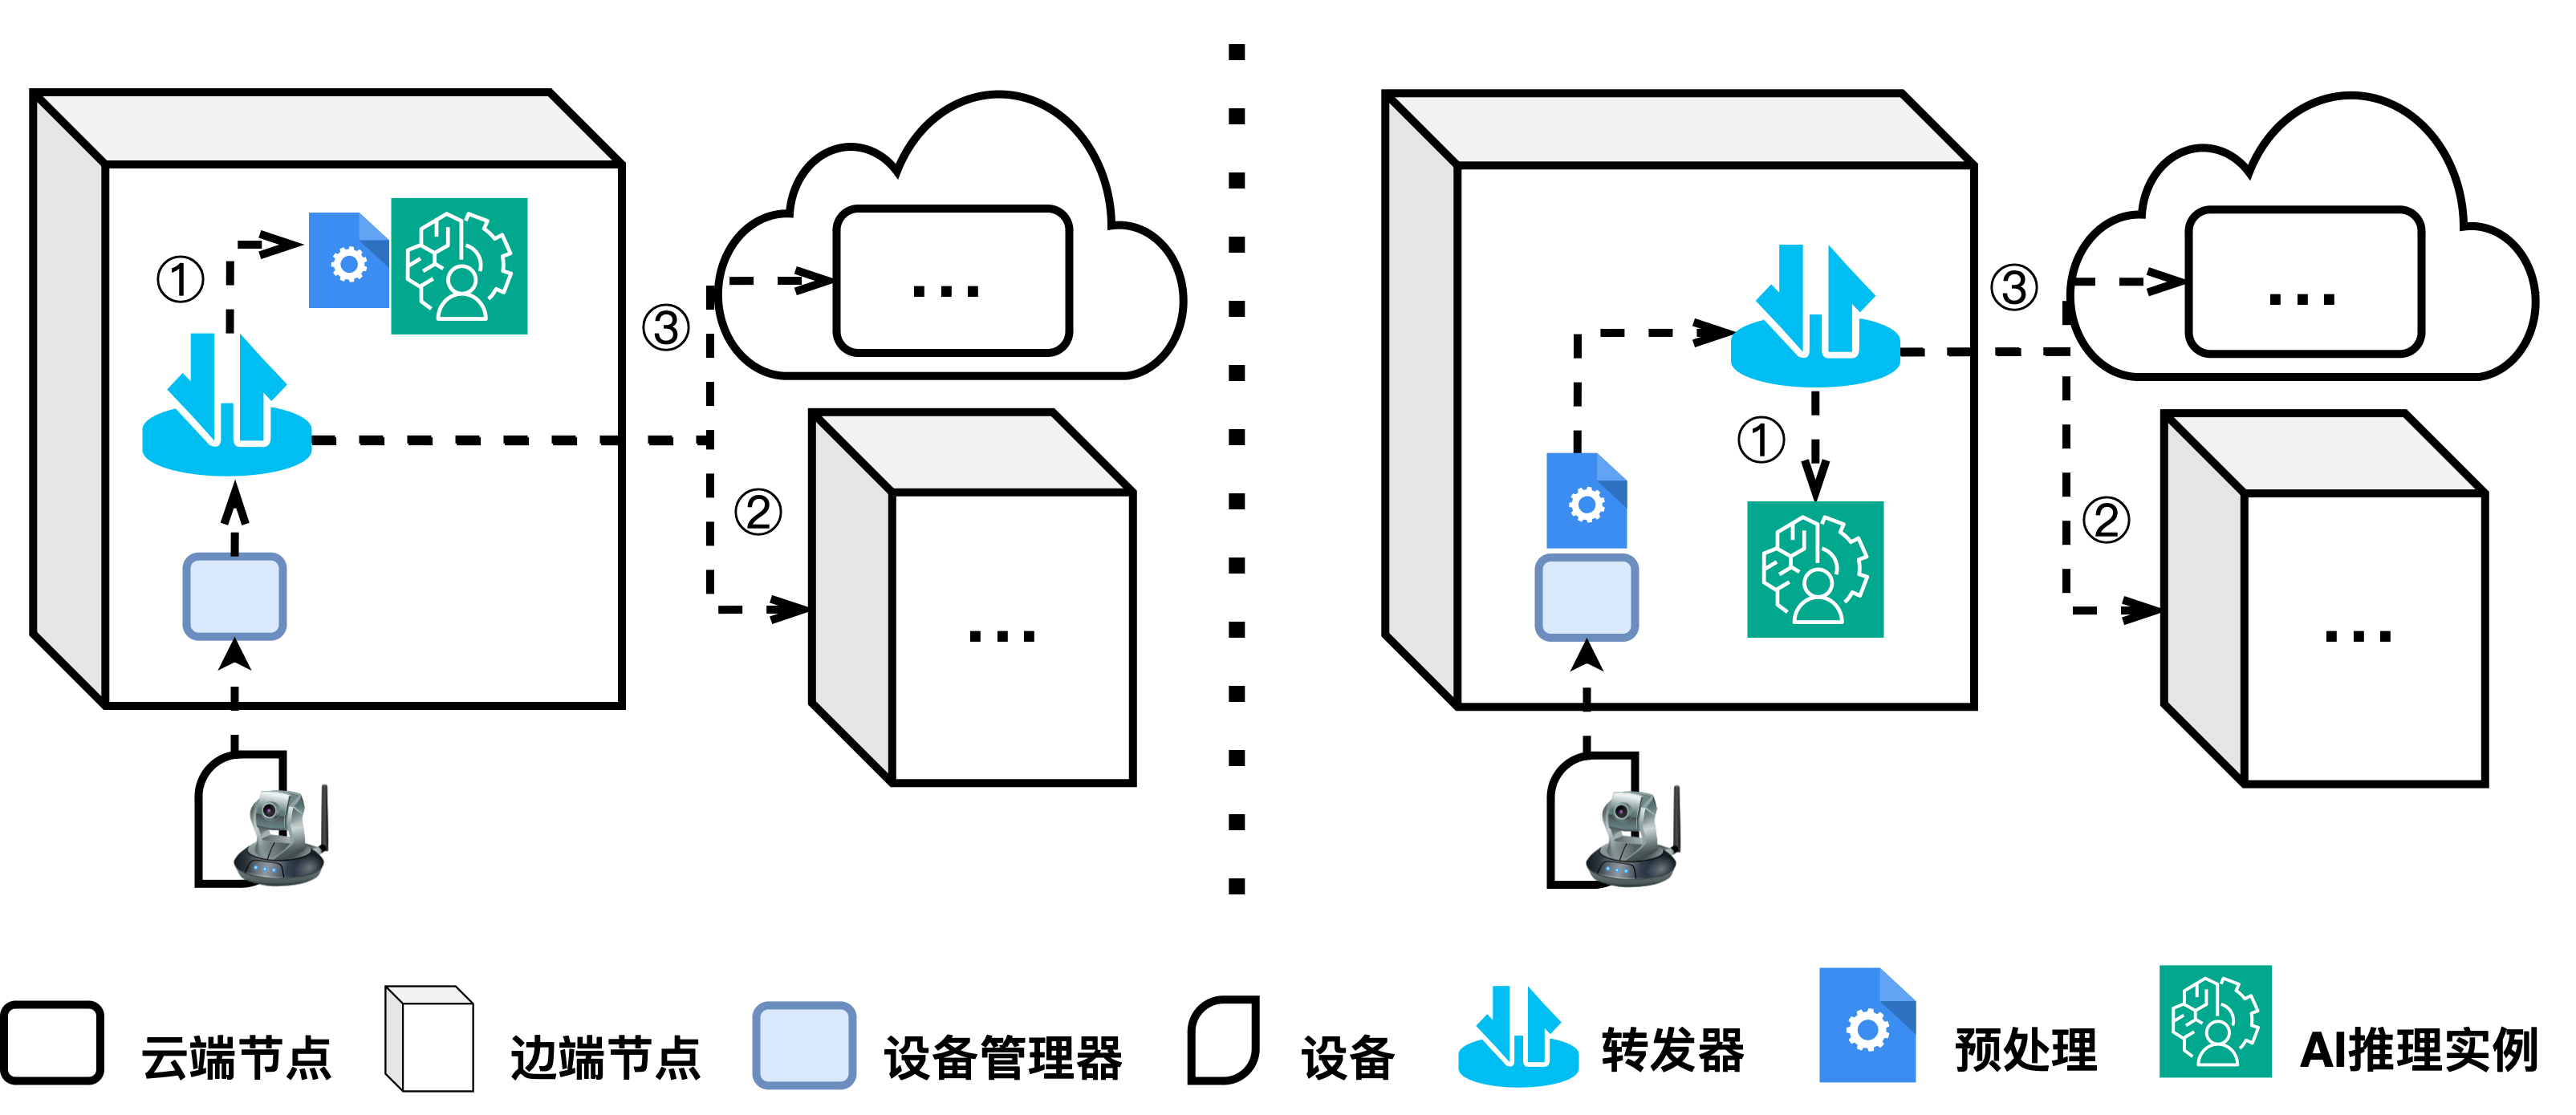
\includegraphics[width=\linewidth]{pics/3-4AI负载.png}
  \caption{云边环境下模型推理实例的端到端处理流程}
  \label{fig:3-4aiload}
\end{figure}

如图\ref{fig:3-4aiload}所示,在云边协同架构中,预处理逻辑的部署位置具有高度灵活性。一种常见的方案是将预处理任务集成到设备管理器中,在数据采集阶段实时完成。这种方式在某些场景下能够有效减少传输至后续环节的数据量,从而降低带宽占用和系统延迟,特别适用于对时效性要求较高的应用。例如,在工业自动化或智能交通系统中,实时处理可以确保关键信息的及时传递。另一种方案则是将预处理任务推迟到模型推理实例中执行。这种设计更适合那些需要结合上下文信息或全局视图进行复杂处理的任务。例如,在医疗监测或环境分析中,可能需要综合多个传感器的数据来进行更全面的分析,此时在云端进行预处理可以利用更强的计算资源和全局数据视图。此外,云边环境中的数据转发器进一步增强了系统的灵活性。数据转发器可以根据实际需求,选择性地传输已预处理的结构化数据或原始数据。这种机制不仅能够在保持数据时效性的同时满足不同场景的需求,还为资源分配和性能优化提供了更多可能性。

% \begin{figure}[ht]
%   \centering
%   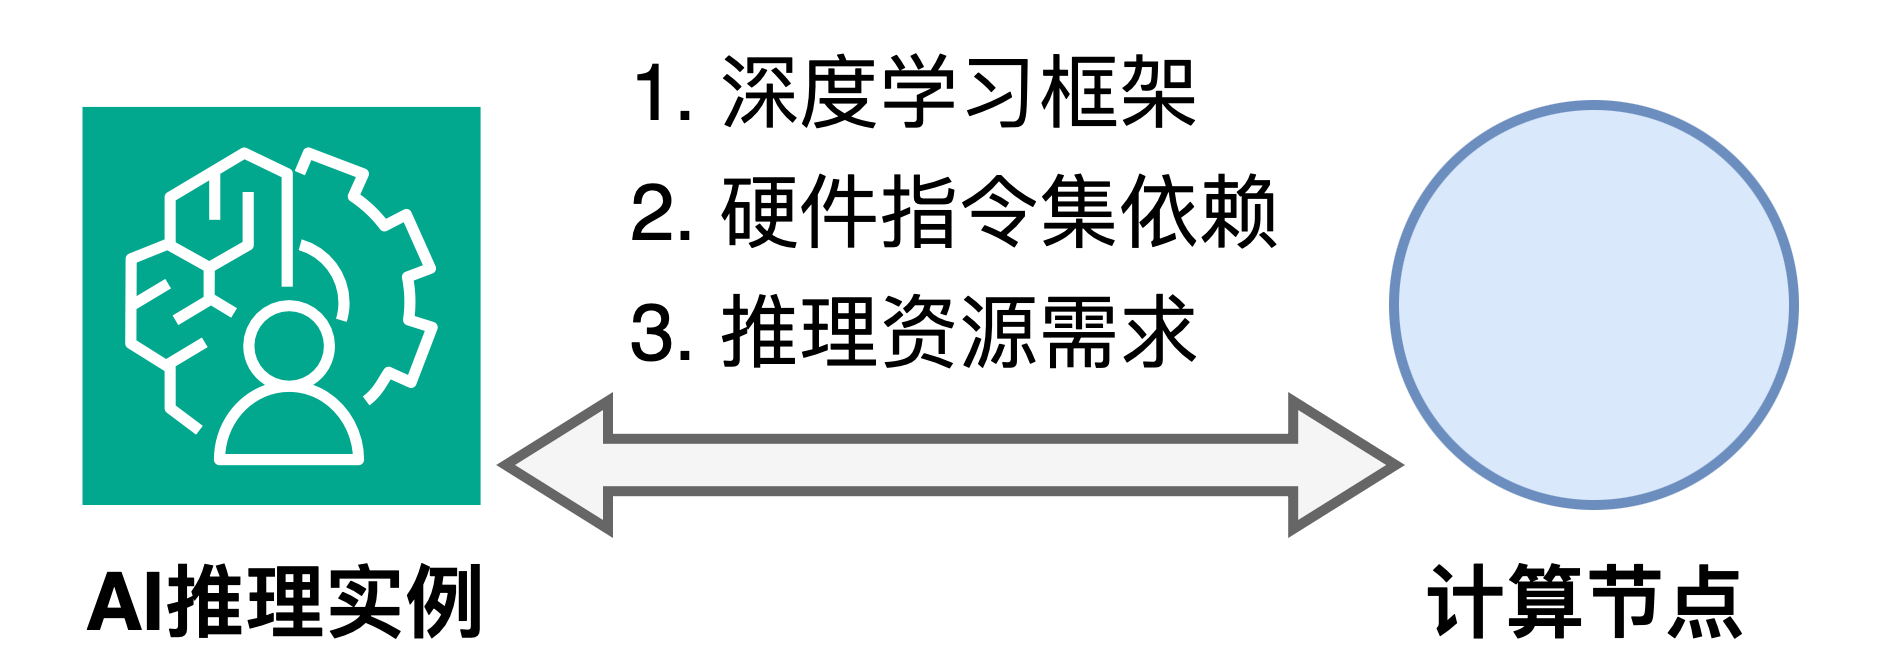
\includegraphics[width=0.5\linewidth]{pics/3-6AI推理实例与计算节点.png}
%   \caption{AI推理实例与计算节点适配关系图}
%   \label{fig:3-6ainode}
% \end{figure}

当经过预处理的数据传递至计算节点后,推理过程即可在对应的AI推理实例上执行。然而,模型推理实例对不同计算节点的适配性存在显著差异,这种差异主要体现在深度学习框架依赖、硬件指令集支持以及推理资源需求等方面。首先,模型通常在特定框架及其版本下开发,而不同计算节点可能未安装所需的框架或版本。此外,许多框架的版本与其对硬件指令集的支持深度绑定,这种绑定关系直接影响模型的部署和运行效率。例如,当前主流框架(如TensorFlow)的最新版本通常默认启用AVX2指令集优化,以大幅提升张量运算性能。然而,在将其部署到不支持AVX2指令的边缘节点时,则需要通过重新编译框架源码或降级至兼容版本来实现正常运行。即便目标节点具备相应的硬件指令集,不同架构(如x86与ARM)对同一指令集的优化程度也可能导致运行效率的显著差异\cite{ren2019performance}。这种硬件架构的异构性要求在部署AI负载时,必须明确其对指令集和架构的具体需求。

其次,资源需求是影响AI负载适配性的另一关键因素。许多大型深度学习模型在设计之初便针对GPU等高性能加速器进行优化,依赖于GPU的大规模并行计算能力。然而,在资源受限的边缘节点上,可能缺乏GPU或其他专用加速器,导致模型无法运行或运行效率低下。同时,为了充分利用节点的计算能力,不同的AI负载实例会根据节点性能配置相应的批处理规模。例如,在高性能云端节点上可以采用较大的批处理规模以提高吞吐量,而在资源受限的边缘节点上则需降低批处理规模以避免资源过载。

\subsection{分层拓扑下的委托推理}

在云边协同的树状拓扑结构下,每一个边缘节点都可能收到来自不同来源的AI推理任务请求。这些任务请求既可能是直接来自终端设备(如传感器、摄像头等)的本地任务请求,也可能是由下一层次的边缘节点传递上来的跨层级任务请求。面对这些任务请求,每个边缘节点需要根据自身的资源状况、任务优先级以及系统整体目标,灵活地调度决策。

\begin{figure}[ht]
  \centering
  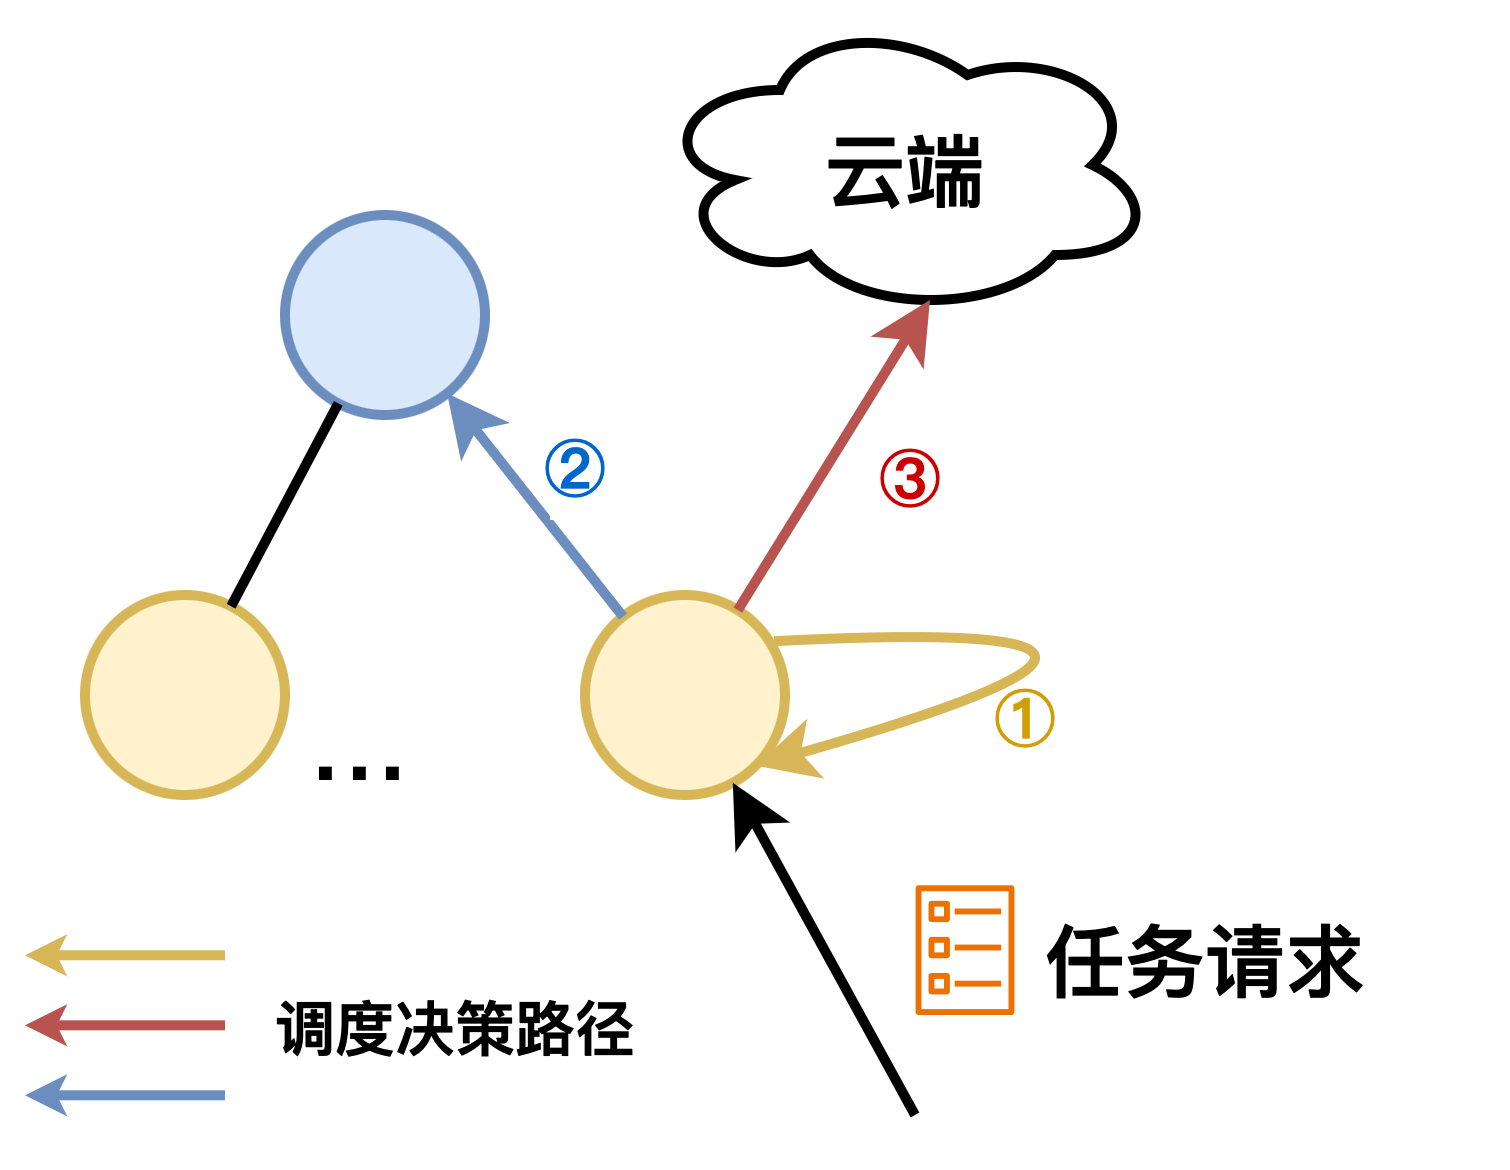
\includegraphics[width=0.45\linewidth]{pics/3-7节点调度.png}
  \caption{边缘节点任务调度}
  \label{fig:3-7node}
\end{figure}

如图\ref{fig:3-7node}所示,在云边协同架构中,任务可以根据需求被灵活调度到不同的位置进行处理。这种调度机制的核心在于根据任务特性、节点资源状况以及系统目标,选择最优的执行路径。当前节点如果具备足够的计算资源,并且任务可以在其子树范围内完成,则可以直接在本地子树中进行处理。需要注意的是,对于与设备直接连接的最低一层边缘节点,其子树实际上就是它自身。这种方式能够显著降低任务执行延迟,同时减少网络带宽占用,特别适合对实时性要求较高的任务。例如,视频监控中的目标检测任务通常可以在靠近摄像头的边缘节点上完成,从而快速响应异常事件。此外,当任务复杂度较高或本地资源不足时,可以选择将任务传递到上一层次的节点进行处理。上层节点通常具有更强的计算能力和更大的存储容量,因此更适合处理那些需要更高性能支持的任务。例如,涉及多源数据融合的任务可能需要汇聚来自多个边缘节点的数据,因此更适合在上层节点完成。对于计算密集型任务或需要全局视角的任务,还可以直接将任务传递到云端进行处理。云端凭借其强大的计算资源和全局数据视图,能够高效完成复杂的推理或分析任务。

\section{面向模型推理的云边协同调度模型}

针对上述架构特征与技术挑战,本文提出了一种面向模型推理的云边协同调度模型,旨在系统性解决云边环境中的模型推理任务调度问题。该模型通过抽象任务特征与系统约束,构建了一个统一的调度框架,以支持多样化的模型推理应用场景。其核心目标包括:首先,明确云边环境的核心组成要素,包括计算节点、网络拓扑、模型推理负载以及终端设备,为模型的设计提供清晰的结构化基础;其次,形式化描述模型推理过程中的关键开销,包括计算开销、通信开销等,从而为后续的调度算法实现奠定坚实的理论基础。

下面给出面向模型推理的云边协同调度模型的形式化定义:

\begin{definition}[面向模型推理的云边协同调度模型]
面向模型推理场景的云边协同调度模型可表示为一个5元组:
\end{definition}

$$
M = (D, E, C, L, B)
$$

其中:

\begin{itemize}
    \item $D = \{d_i\}_{i=1}^n$ 表示终端设备集合,其中每个终端设备$d_i$用于物联网数据采集,具体定义详见定义\ref{def:device}。
    \item $E = \{e_j\}_{j=1}^m$ 表示边缘节点集合,每个节点$e_j$具有有限计算资源,部署在网络边缘靠近终端设备的位置,具有低时延响应能力。
    \item $C = \{c_q\}_{q=1}^r$ 表示云端节点集合,每个节点$c_q$配备高性能计算资源,适用于计算密集的大规模模型推理或模型训练。
    \item $L = \{l_s\}_{s=1}^u$ 表示模型推理实例集合,其中每个模型负载实例$l_s$负责处理终端设备产生的实时流数据并执行推理任务,具体定义详见定义\ref{def:aimodel}。
    \item $B \in \mathbb{R}^{\mu \times \mu}$ 为带宽矩阵,其中$\mu=m+r$,表示云边环境下的所有节点数量,元素 $b_{pq}$ 表示节点 $p$ 到节点 $q$ 的有效带宽。
\end{itemize}

为了更清晰地描述模型的动态运行特性,本文将云边平台的运行时间划分为一系列等长时间窗 $\{t_\omega\}_{\omega=1}^\infty$。其中,第 $\omega$ 个调度时间窗定义为 $t_\omega = [\tau_\omega, \tau_\omega + \Delta t)$,$\Delta t$ 表示时间窗的长度参数。在此基础上,后续章节将进一步展开对计算节点、终端设备、模型推理实例的详细分析。

\subsection{计算节点}

在云边协同计算架构中,计算节点作为任务处理和资源分配的核心实体,承担着数据处理、存储以及通信的关键职能。计算节点集合$V = E \cup C$涵盖边缘节点集合$E$与云端节点集合$C$,总共包含$\mu=m+r$个计算节点。由于云边环境中的节点具有异构化的资源供给和硬件架构特性,为了实现高效的模型推理实例部署,需要对每个节点的资源供给能力、硬件架构特性和计算能力进行量化分析。这种量化过程能够为任务调度和资源优化提供科学依据,从而提升整体系统的性能与效率。

下面给出计算节点的形式化定义:

\begin{definition}[计算节点]
\label{def:node}
计算节点 $v_j \in V$ 可表示为一个 3 元组:
\end{definition}

$$
v_j = (R_j,\, Arch_j,\, Perf_j ,\, Tree_j)
$$

其中:
\begin{itemize}
    \item $R_j = \{r^{k}_j\}_{k=1}^w$ 表示资源供给向量,其中 $r^{(k)}_j \in \mathbb{R}^+$ 表示第 $k$ 类资源总量。
    \item $Arch_j \in H$ 表示硬件架构,$H$ 为硬件架构类型枚举集。
    \item $Perf_j \in \mathbb{R}^+$ 表示计算性能,单位为每秒浮点运算次数(FLOPS)。
    \item $Tree_j \subseteq V$ 表示当前节点的子节点集合,用于描述树状拓扑结构中的下一层节点关系。
\end{itemize}

通过引入 $Tree_j$,可以明确地表达云边协同架构中计算节点的层级关系。对于直接连接终端设备的最低层边缘节点,其子节点集合 $Tree_j = \emptyset$,即没有下一层节点;而对于其他中间层或顶层节点(如云端节点),其子节点集合 $Tree_j$ 包含所有直连的下一层节点。这种树状拓扑结构的设计不仅简化了系统管理复杂度,还为任务调度提供了重要的参考信息。

\subsection{终端设备}

在物联网架构下,终端设备作为数据采集的核心单元,其行为特性可以从静态属性和动态数据采集两个维度进行刻画。静态属性描述了设备的固有能力与接口规范,这些属性在设计阶段确定,通常不可更改,能够表征设备类型;而动态数据采集则关注设备运行时的数据生成过程,包括采样频率、传输速率等特性,这些特性随设备的工作状态而波动,反映着设备实时交互与响应的能力。

下面给出终端设备的形式化定义:

\begin{definition}[终端设备]
\label{def:device}
终端设备 $d_i \in D$ 可表示为一个 2 元组:
\end{definition}

$$
d_i = (\Omega_\beta, g_\beta)
$$

其中:
\begin{itemize}
    \item $\Omega_\beta = (X^{(k)}_\beta)_{k=1}^{\zeta}$ 表示静态属性集合($\zeta \in \mathbb{N}^+$ 为属性维度),表征设备的物理特性。
    \item $g_\beta(t)$ 表示瞬时数据采集频率函数,需满足 Lipschitz 连续条件:
        \begin{equation}
        \exists K_\beta > 0,\ \forall t_1, t_2 \in \mathbb{R},\ |g_\beta(t_2) - g_\beta(t_1)| \leq K_\beta |t_2 - t_1|
        \end{equation}
        其中 $K_\beta$ 表示设备物理特性决定的最大调节速率。
\end{itemize}

终端设备的静态属性体现了显著的类型特异性,这种特异性源于设备在功能设计和物理实现上的差异。例如,视觉设备的静态属性通常包括分辨率、位深度、压缩算法及总线配置等量化参数;温度传感器则包含量程范围和测量精度等物理特性参数。为简化论述,本文假设初始场景中所有终端设备属于单一类型,该假设可通过服务发现机制扩展至多设备场景。

这些静态属性不仅表征了设备的基础能力,还为数据量计算提供了关键依据。以视觉设备为例,其单帧数据量可通过分辨率与位深度的乘积初步估算,并结合压缩率修正得出精确值。本文采用$\varsigma_\beta \in \mathbb{R}^+$ 表示单次数据采集量,通过标准化转换函数计算:

\begin{equation}
\varsigma_\beta = \varphi(\Phi_\beta) = \prod_{k=1}^{\zeta} f_k(X^{(k)}_\beta)
\end{equation}

其中 $f_k: P \to \mathbb{R}^+$ 为预定义的属性量化函数。进一步地,终端设备 $d_i$ 的瞬时数据采集流量 $G_i(t)$ 由瞬时数据采集频率 $g_i(t)$ 和单次采集量 $\varsigma_\beta$ 共同决定,具体表达式为:

\begin{equation}
G_i(t) = g_i(t) \cdot \varsigma_\beta
\end{equation}

\subsection{模型推理实例}

在异构环境下的模型推理实例部署中,框架兼容性、指令集支持以及资源适配性等问题构成了显著挑战。为了有效应对这些挑战,本文对模型推理实例进行形式化描述,明确其关键属性及其对运行环境的具体需求。这种形式化的定义不仅能够量化模型推理实例对深度学习框架、硬件架构和资源的需求,还为评估其在不同计算节点上的适配性提供了理论基础。

下面给出模型推理实例的形式化定义:

\begin{definition}[模型推理实例] 
\label{def:aimodel}
AI 推理实例$l_s \in L$ 可表示为一个 5 元组:
\end{definition}

$$
l_s = (F_s,\, A_s,\, R_s,\, \gamma_s,\, \varpi_s)
$$

其中:
\begin{itemize}
    \item $F_s \in \mathbb{S}$ 表示支持的深度学习框架,$\mathbb{S}$为云边平台支持的深度学习框架枚举集。
    \item $A_s \subseteq H$ 表示硬件架构需求集合,$H$为硬件架构类型枚举集。
    \item $R_s = \{r^{(k)}_s\}_{k=1}^w$ 表示资源需求向量,其中$r^{(k)}_s \in \mathbb{R}^+$对应第$k$类资源的最小需求。
    \item $batch_s \in \mathbb{Z}^+$ 表示批处理规模,满足$batch_s \leq \lfloor \frac{R_s}{\delta_s} \rfloor$,其中$R_s$为设备内存容量,$\delta_s$为单样本内存占用量。
    \item $\varpi_s \in \mathbb{R}^+$ 表示单次推理运算量,单位为浮点运算次数(FLOPs)。
\end{itemize}

在明确了模型推理实例的形式化定义后,在目标节点 $v_j$上部署模型推理实例 $l_s$ 需要确保资源供给和硬件架构相匹配。具体而言,需满足以下条件:

\begin{equation}
R_j \geq R_s, \quad A_s \subseteq Arch_j
\end{equation}

其中,$R_j$ 和 $R_s$ 分别表示节点 $v_j$ 的资源供给向量和模型推理实例 $l_s$ 的资源需求向量;$Arch_j$ 和 $A_s$ 分别表示节点 $v_j$ 的硬件架构和模型推理实例 $l_s$ 的硬件架构需求。在节点$v_j$上成功部署模型推理实例$l_s$之后,可以通过推理时间预测函数$\text{Latency}_{\text{inf}}$来量化单次推理延迟,该函数可表示为:

\begin{equation}
\text{Latency}_{\text{inf}}(l_s, v_j)= \frac{\varpi_s}{Perf_j}
\end{equation}

其中,$\varpi_s$ 为模型推理实例$l_s$的单次推理运算量,$Perf_j$为节点$v_j$的计算性能。在明确了单次推理延迟$\text{Latency}_{\text{inf}}$之后,对于任意时间窗$t_\omega = [\tau_\omega, \tau_\omega + \Delta t)$,节点$v_j$可承载的模型推理实例$l_s$的最大吞吐量$Q(l_s, v_j, t_\omega)$可以通过以下公式计算:

\begin{equation}
Q(l_s, v_j, t_\omega) = \left\lfloor \frac{\Delta t}{\text{Latency}_{\text{inf}}(l_s, v_j)} \right\rfloor \cdot batch_s
\end{equation}

其中,$batch_s$表示模型推理实例$l_s$的批处理规模。该指标$Q(l_s, v_j, t_\omega)$表示节点$v_j$在时间窗$t_\omega$内对模型推理实例$l_s$的最大服务容量,是衡量节点资源利用率和服务能力的重要参考。每一个 AI 推理实例 $l_s$ 在时间窗 $t_\omega$ 中都有可能已经被调度分配了对应的任务请求。因此,本文用 $C(l_s, v_j, t_\omega)$ 表示节点 $v_j$ 在时间窗 $t_\omega$ 内剩余的可用容量。这个剩余容量可以表示为:

\begin{equation}
C(l_s, v_j, t_\omega) = Q(l_s, v_j, t_\omega) - \text{AllocatedTasks}(l_s, v_j, t_\omega)
\end{equation}

其中,$\text{AllocatedTasks}(l_s, v_j, t_\omega)$ 表示在时间窗 $t_\omega$ 已经分配给节点 $v_j$ 的模型推理实例 $l_s$ 的任务数量。在实际部署过程中,$Q(l_s, v_j, t_\omega)$和$C(l_s, v_j, t_\omega)$的指标由系统监控服务动态维护,并作为分层委托调度决策过程的核心输入之一。调度器需确保分配至节点$v_j$的模型推理实例$l_s$的请求速率不超过其最大吞吐量$Q(l_s, v_j, t_\omega)$,从而避免因计算资源过载而导致的排队延迟或任务失败。


\subsection{流式数据分流机制}

在云边协同环境中,终端设备产生的实时流式数据是整个系统调度的核心驱动因素。根据定义\ref{def:device}中终端设备的形式化描述,可以推导出在时间窗$t_\omega = [\tau_\omega, \tau_\omega + \Delta t)$内,设备 $d_i$ 的数据采集总量为$g_i^{t_\omega} = \int_{\tau_\omega}^{\tau_\omega + \Delta t} g_i(t) \, dt$,其中$g_i(t)$ 表示终端设备 $d_i$ 在时刻 $t$ 的瞬时数据采集频率。为实现动态负载均衡,各级调度器需将流式数据按需分发至适配的计算节点,这一过程通过流式数据分流机制实现。

下面给出流式数据分流函数的形式化定义:

\begin{definition}[流式数据分流函数]
流式数据分流可定义为函数$\zeta$:
\end{definition}

$$
\zeta: g_i^{t_\omega} \to \left( g_{i1}^{t_\omega},\ g_{i2}^{t_\omega},\ \dots,\ g_{i\mu}^{t_\omega} \right) \ \text{with} \ Z_i^{t_\omega} = \{z_{ij}^{t_\omega}\}_{j=1}^\mu
$$

其中:
\begin{itemize}
    \item $g_i^{t_\omega}$表示时间窗$t_\omega$内设备$d_i$的数据总量。
    \item $g_{ij}^{t_\omega}$表示分流给计算节点$v_j$的数据子流,满足$\sum\limits_{j=1}^\mu g_{ij}^{t_\omega} = g_i^{t_\omega}$,且子流大小与比例变量满足$g_{ij}^{t_\omega} = z_{ij}^{t_\omega} \cdot g_i^{t_\omega}$。
    \item 分流比例集合$Z_i^{t_\omega} = \{z_{ij}^{t_\omega}\}_{j=1}^\mu$需满足:$\forall j \in \{1,\dots,\mu\},\ 0 \leq z_{ij}^{t_\omega} \leq 1$,且$\sum\limits_{j=1}^\mu z_{ij}^{t_\omega} = 1$。
\end{itemize}

该函数通过分流变量$Z_i^{t_\omega}$将终端设备产生的数据流划分为$\mu$个计算节点关联的数据子流。在实际部署中,数据流的跨节点转发不可避免地引入了传输时延。例如,假设节点$v_j$上的设备$d_i$的所有采集数据均需转发至计算节点$v_{j'}$,其传输时延可由下式计算:

\begin{equation}
\text{Latency}_\text{trans}=\frac{G_i}{b_{jj'}}
\end{equation}

其中,\(G_i\)代表数据流量,$b_{jj'}$是节点$v_j$至$v_{j'}$间的带宽。

\section{面向模型推理的云边协同调度算法}

面向模型推理的云边协同调度策略在不同层次上优化了多个目标。为了实现这些目标,需要通过高效的数据分流,即将流式数据合理地分配给不同的节点,以确保计算资源的有效利用和任务处理的高效性。为此,本文设计了一种请求队列机制。该机制能够有效识别并区分本地生成的数据与来自其他节点的数据,从而精细控制数据流动方向。这不仅支持更复杂的任务调度算法,还提高了系统的响应速度和服务质量。

\begin{figure}[h]
  \centering
  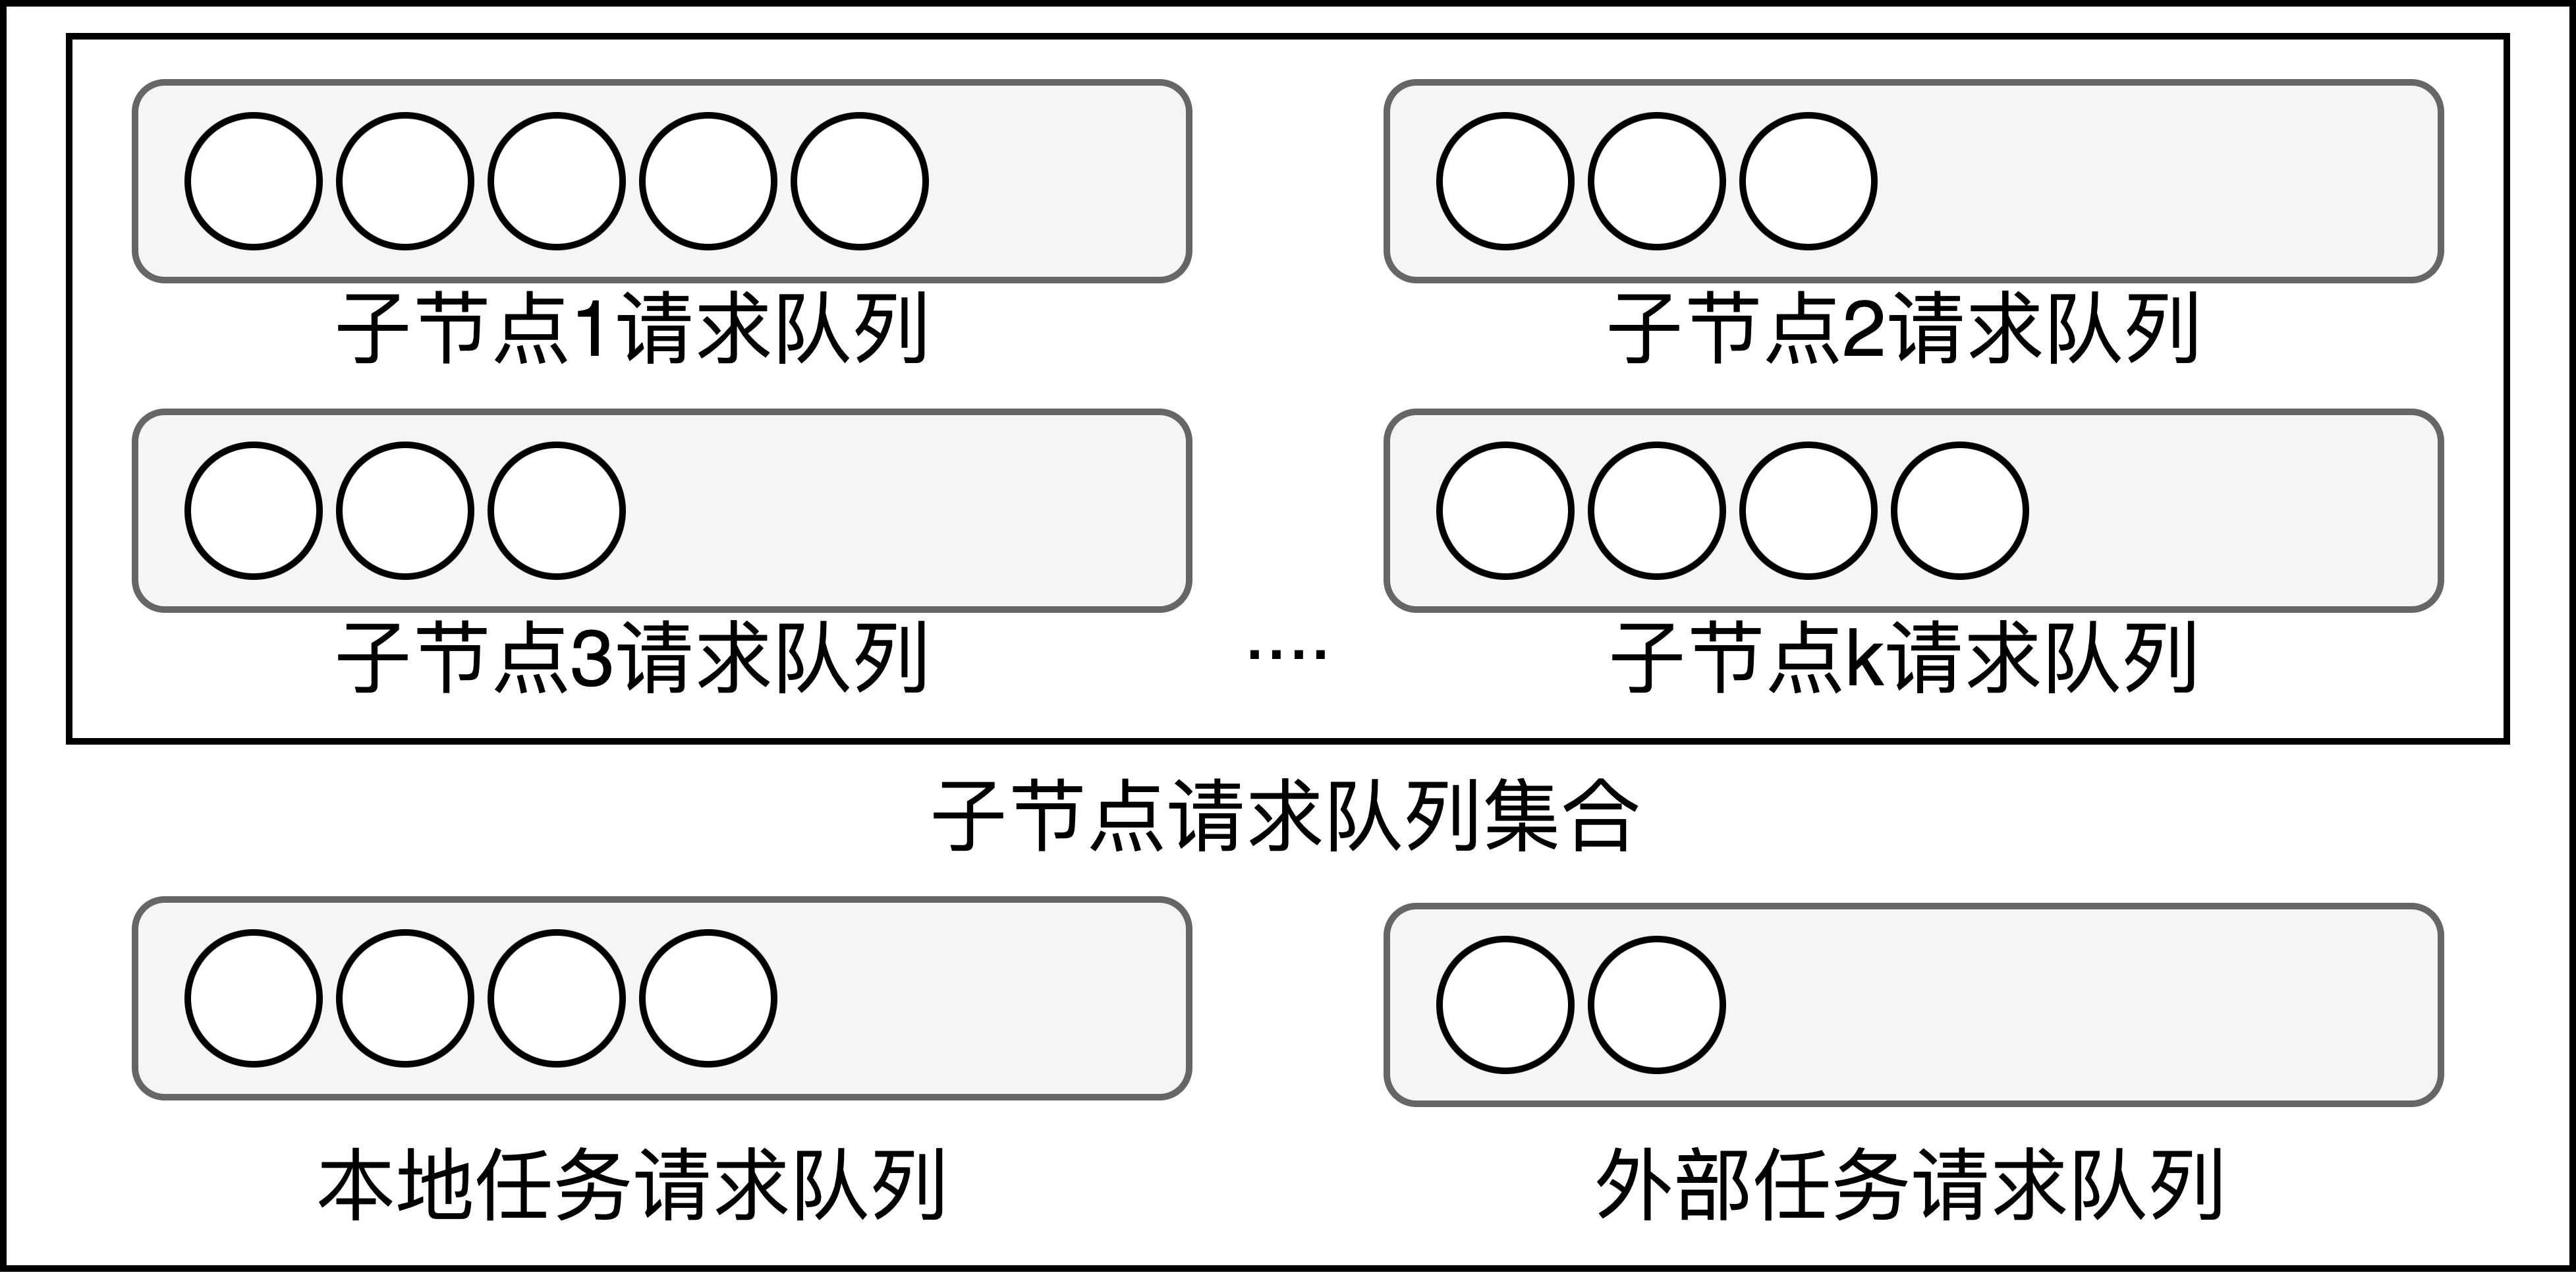
\includegraphics[width=0.75\linewidth]{pics/3-11集群调度.png}
  \caption{节点调度任务队列}
  \label{fig:3-11cluster}
\end{figure}

如图\ref{fig:3-11cluster}所示,每个计算节点都维护着三种类型的任务队列:自身关联设备产生的数据流任务队列、所有下级节点的任务队列信息以及来自外部的任务队列信息。对于直接与设备相连的最底层边缘节点而言,其子节点任务队列为空。在执行任务调度时,各节点的调度器会优先处理本地生成的数据流任务及下级节点的任务请求。只有当这些内部任务得到妥善安排后,才会考虑处理外部节点提出的任务请求。这样可以确保本地数据流能够优先获得所需的计算资源。

在实际调度过程中,边缘节点和云端节点采用了不同的策略以适应各自的特点。边缘节点由于资源有限且需减少跨节点传输开销,会优先处理单次采集量最大的任务,即采用最大数据量优先(Large Data First Out, LDFO)策略。这可以有效降低频繁小规模数据传输带来的额外成本,并提高本地数据处理效率。相比之下,云端节点具备更强的计算能力和全局视角,其调度策略侧重于最大化设备处理能力。为此,云端会优先处理最小的碎片任务,即采用最小任务优先(Small Task First Out, STFO)策略,从而确保尽可能多的设备请求得到完整处理,提升系统整体的吞吐量和资源利用率。

\begin{breakablealgorithm}
\caption{面向模型推理的云边协同调度算法}
\label{alg:cluster_scheduling}
\begin{algorithmic}[1]
\REQUIRE  
  待调度数据流及单次采集量集合$\{(g_i, \varsigma_{\beta_i})\}_{i=1}^p$, 
  计算节点集合$V$的队列剩余容量$\{C^{t_\omega}_j\}_{v_j \in V}$, 带宽矩阵$B$, 当前节点$v_c$的子树拓扑$Tree_{v_c}$ \\ \COMMENT{如果是 Edge mode,$g_i$可以分为本地数据流$g_i^{\text{loc}}$和外部数据流$g_i^{\text{ext}}$}
\ENSURE  
  数据流到计算节点的分流比例集合$\{z_{ij}^{t_\omega}\}$
  
\STATE Initialize $z_{ij}^{t_\omega} \leftarrow 0,\ \forall g_i \in F_k, v_j \in Tree_{v_c}$  

\IF{Edge mode}
\STATE $Q \leftarrow \textsc{Sort}(\{g_i^{\text{loc}}\}, \varsigma_{\beta_i} \downarrow) \cup \textsc{Sort}(\{g_j^{\text{ext}}\}, \varsigma_{\beta_j} \downarrow)$
  \\ \COMMENT{本地数据流$g_i^{\text{loc}}$优先,按单次数据量$\varsigma_{\beta_i}$降序}
\ELSIF{Cloud mode}
\STATE Sort $Q \leftarrow \textsc{Sort}( g_i, \varsigma_{\beta_i} \uparrow)$ 
    \COMMENT{按剩余数据量升序排列}
\ENDIF

\FOR{$(g_i, \varsigma_{\beta_i}) \in Q$} 
  \STATE Filter $N_i \leftarrow \{v_j \in Tree_{v_c} \mid A_s \subseteq Arch_j \wedge R_j \geq R_s \wedge C^{t_\omega}_j > 0\}$  
    \\ \COMMENT{筛选兼容且有剩余容量的子节点}
  \STATE Compute $\Theta_j = \frac{\varsigma_{\beta_i}{B}(v_c,v_j)} + \frac{\varpi_s}{Perf_j}$
  \STATE Order $M_i \leftarrow \textsc{Sort}(N_i, \Theta_j \uparrow)$  
    \COMMENT{按端到端时延升序排序}
  \STATE Set $r_i \leftarrow g_{i,\text{res}^{t_\omega}}$

  \WHILE{$r_i > 0$ \AND $M_i \neq \emptyset$}
    \STATE Dequeue $v_j \leftarrow M_i.\textsc{Dequeue}()$
    \STATE Calculate $a_j \leftarrow C^{t_\omega}_j - \sum_{f_k \in F_k} z_{kj}^{t_\omega} \cdot g_{k,\text{res}^{t_\omega}}$
    
    \IF{$a_j \geq r_i$}
      \STATE Assign $z_{ij}^{t_\omega} \leftarrow r_i / g_{i,\text{res}}^{t_\omega}$  
        \COMMENT{全量分配给当前节点}
      \STATE Update $C^{t_\omega}_j \leftarrow C^{t_\omega}_j - r_i$
      \STATE Reset $r_i \leftarrow 0$
    \ELSE
      \STATE Assign $z_{ij}^{t_\omega} \leftarrow a_j / g_{i,\text{res}}^{t_\omega}$  
        \COMMENT{按剩余容量比例分配}
      \STATE Update $C^{t_\omega}_j \leftarrow 0$
      \STATE Reduce $r_i \leftarrow r_i - a_j$
    \ENDIF
  \ENDWHILE
\ENDFOR
\RETURN $\{z_{ij}^{t_\omega}\}$
\end{algorithmic}
\end{breakablealgorithm}

基于上述分析,本文提出了一种结合贪心策略与多维度优先级队列的云边协同AI推理调度算法。该算法首先根据设备单次数据采集量或剩余数据量对流式数据进行优先级排序,构建初始优先级队列。在此基础上,针对每条流式数据,算法筛选出集群中具有剩余计算队列容量的候选节点,并进一步依据端到端时延建立时延优先队列。通过引入时延敏感度感知机制,算法有效降低了节点之间调度的总时延,尽可能满足任务的时延约束要求。此外,算法采用动态分配策略,在候选节点间按照剩余容量比例分配数据流。这一设计不仅避免了单一节点过载的问题,还最大化了集群内部计算资源的利用率。为了进一步优化性能,该算法还引入了自适应调整机制,根据实时网络状况和计算负载动态调整优先级队列和调度策略。这种自适应性确保了算法在不同场景下的鲁棒性和灵活性。通过上述机制,该算法在保证服务质量的同时实现了高效的资源调度与任务分配,具体流程详见算法\ref{alg:cluster_scheduling}。

算法\ref{alg:cluster_scheduling}的总体时间复杂度为$O(|F_k| \log |F_k| + |F_k| \cdot |Tree_c| \log |Tree_c|)$,其中$|F_k|$表示待调度数据流的数量,$|Tree_c|$表示当前节点$v_c$的子树拓扑中的节点数。具体来说,生成数据流优先级队列时间复杂度为$O(|F_k| \log |F_k|)$;节点匹配阶段的时间复杂度为$O(|F_k| \cdot |Tree_c| \log |Tree_c|)$;分配阶段总时间复杂度为$O(|F_k| \cdot \langle d \rangle)$,在最坏情况下可以简化为$O(|F_k|)$,其中$\langle d \rangle$表示平均迭代深度且满足$\langle d \rangle \leq \min(|F_k|, |Tree_c|)$。这种时间复杂度使得算法在大规模数据流和节点数量的情况下仍能保持较高的效率,特别适用于动态和复杂的云边协同环境。

算法\ref{alg:cluster_scheduling}的总体空间复杂度为$O(|Tree_c| \cdot |F_k| + \max(|F_k|, |Tree_c|))$。其中,分流比例矩阵$Z^{t_\omega}$的空间复杂度为$O(|Tree_c| \cdot |F_k|)$,临时数据结构的空间复杂度为$O(\max(|F_k|, |Tree_c|))$。这种空间复杂度设计确保了算法在处理大量数据流时能够高效利用内存资源,同时保持良好的扩展性和可维护性。

\section{本章小结}

本章系统地探讨了面向模型推理的云边协同调度。首先,介绍了云边协同的拓扑结构、模型推理的云边协同场景及分层拓扑下的委托推理,清晰阐释了该环境的复杂性和挑战。基于此,本章提出了一种面向模型推理的云边协同调度模型。该模型详细定义了终端设备、计算节点和模型推理实例的关键组件,包括终端设备的静态属性和动态数据采集特性、计算节点的资源供给能力和硬件架构,以及模型推理实例的部署需求。此外,模型量化了调度过程中的核心开销,为后续的调度算法提供了坚实的理论基础。在此基础上,本章设计并实现了一种结合贪心策略与多维度优先级队列的调度算法。该算法通过优先级排序、候选节点筛选、时延敏感度感知机制和动态分配策略,有效降低了总时延并最大化了资源利用率。算法还引入了自适应调整机制,根据实时网络状况和计算负载动态调整调度策略,确保了算法在不同场景下的鲁棒性和灵活性。
